
%(BEGIN_QUESTION)
% Copyright 2011, Tony R. Kuphaldt, released under the Creative Commons Attribution License (v 1.0)
% This means you may do almost anything with this work of mine, so long as you give me proper credit

Read and outline the ``Fresnel Zones'' subsection of the ``Radio Systems'' section of the ``Wireless Instrumentation'' chapter in your {\it Lessons In Industrial Instrumentation} textbook.  Note the page numbers where important illustrations, photographs, equations, tables, and other relevant details are found.  Prepare to thoughtfully discuss with your instructor and classmates the concepts and examples explored in this reading.

\underbar{file i00549}
%(END_QUESTION)





%(BEGIN_ANSWER)


%(END_ANSWER)





%(BEGIN_NOTES)

RF energy does not follow a straight-line path from transmitting antenna to receiving antenna, even with the most focused antenna.  Instead, we must think of it as occupying a series of oblong spaces called {\it Fresnel zones}.  Fresnel zone radius is calculated as such:

$$r = \sqrt{{n \lambda d_1 d_2} \over D}$$

\noindent
Where,

$r$ = Radius of Fresnel zone at the point of interest

$n$ = Fresnel zone number (an integer value, with 1 representing the first zone)

$d_1$ = Distance between one antenna and the point of interest

$d_2$ = Distance between the other antenna and the point of interest

$D$ = Distance between both antennas

$$\includegraphics[width=15.5cm]{i00549x01.eps}$$

For microwave RF, the goal is to have the inner-most Fresnel zone ($n=1$) no more than 40\% obstructed.  A good goal in RF system design is to avoid any interference within zone 1 at all.  This is what free ``line of sight'' really means: that the entire inner Fresnel zone is free from interefence (including interference from the earth).








\vskip 20pt \vbox{\hrule \hbox{\strut \vrule{} {\bf Suggestions for Socratic discussion} \vrule} \hrule}

\begin{itemize}
\item{} Explain what a {\it Fresnel zone} is, and why it is important to RF link calculations.
\item{} Does the width of a Fresnel zone increase, decrease, or remain the same as signal frequency increases?
\item{} Does the width of a Fresnel zone increase, decrease, or remain the same as signal frequency decreases?
\item{} Does the width of a Fresnel zone increase, decrease, or remain the distance between antennas increases?
\item{} Does the width of a Fresnel zone increase, decrease, or remain the distance between antennas decreases?
\end{itemize}







\vfil \eject

\noindent
{\bf Prep Quiz:}

As the frequency of a radio signal increases, its Fresnel zone will do what (all other things remaining the same)?

\begin{itemize}
\item{} There will be no effect on the Fresnel zone resulting from a frequency change
\vskip 5pt 
\item{} The maximum width of the Fresnel zone will increase (become fatter)
\vskip 5pt 
\item{} The end-to-end length of the Fresnel zone will increase (become longer)
\vskip 5pt 
\item{} The maximum width of the Fresnel zone will decrease (become skinnier)
\vskip 5pt 
\item{} The end-to-end length of the Fresnel zone will decrease (become shorter)
\vskip 5pt 
\item{} The power density will decrease (the RF energy will ``spread'' more)
\end{itemize}



\vfil \eject

\noindent
{\bf Summary Quiz:}

Calculate the {\it maximum total width} of the first Fresnel zone for two radio antennas operating at 2.4 GHz, separated by a distance of 1400 meters:

\begin{itemize}
\item{} 10.80 meters
\vskip 5pt 
\item{} 43.72 meters
\vskip 5pt 
\item{} 6.612 meters
\vskip 5pt 
\item{} 87.44 meters
\vskip 5pt 
\item{} 21.59 meters
\vskip 5pt 
\item{} 13.22 meters
\end{itemize}


%INDEX% Reading assignment: Lessons In Industrial Instrumentation, AC Electricity (antennas -- Fresnel zones)

%(END_NOTES)


